\begin{figure}[!t]
\centering
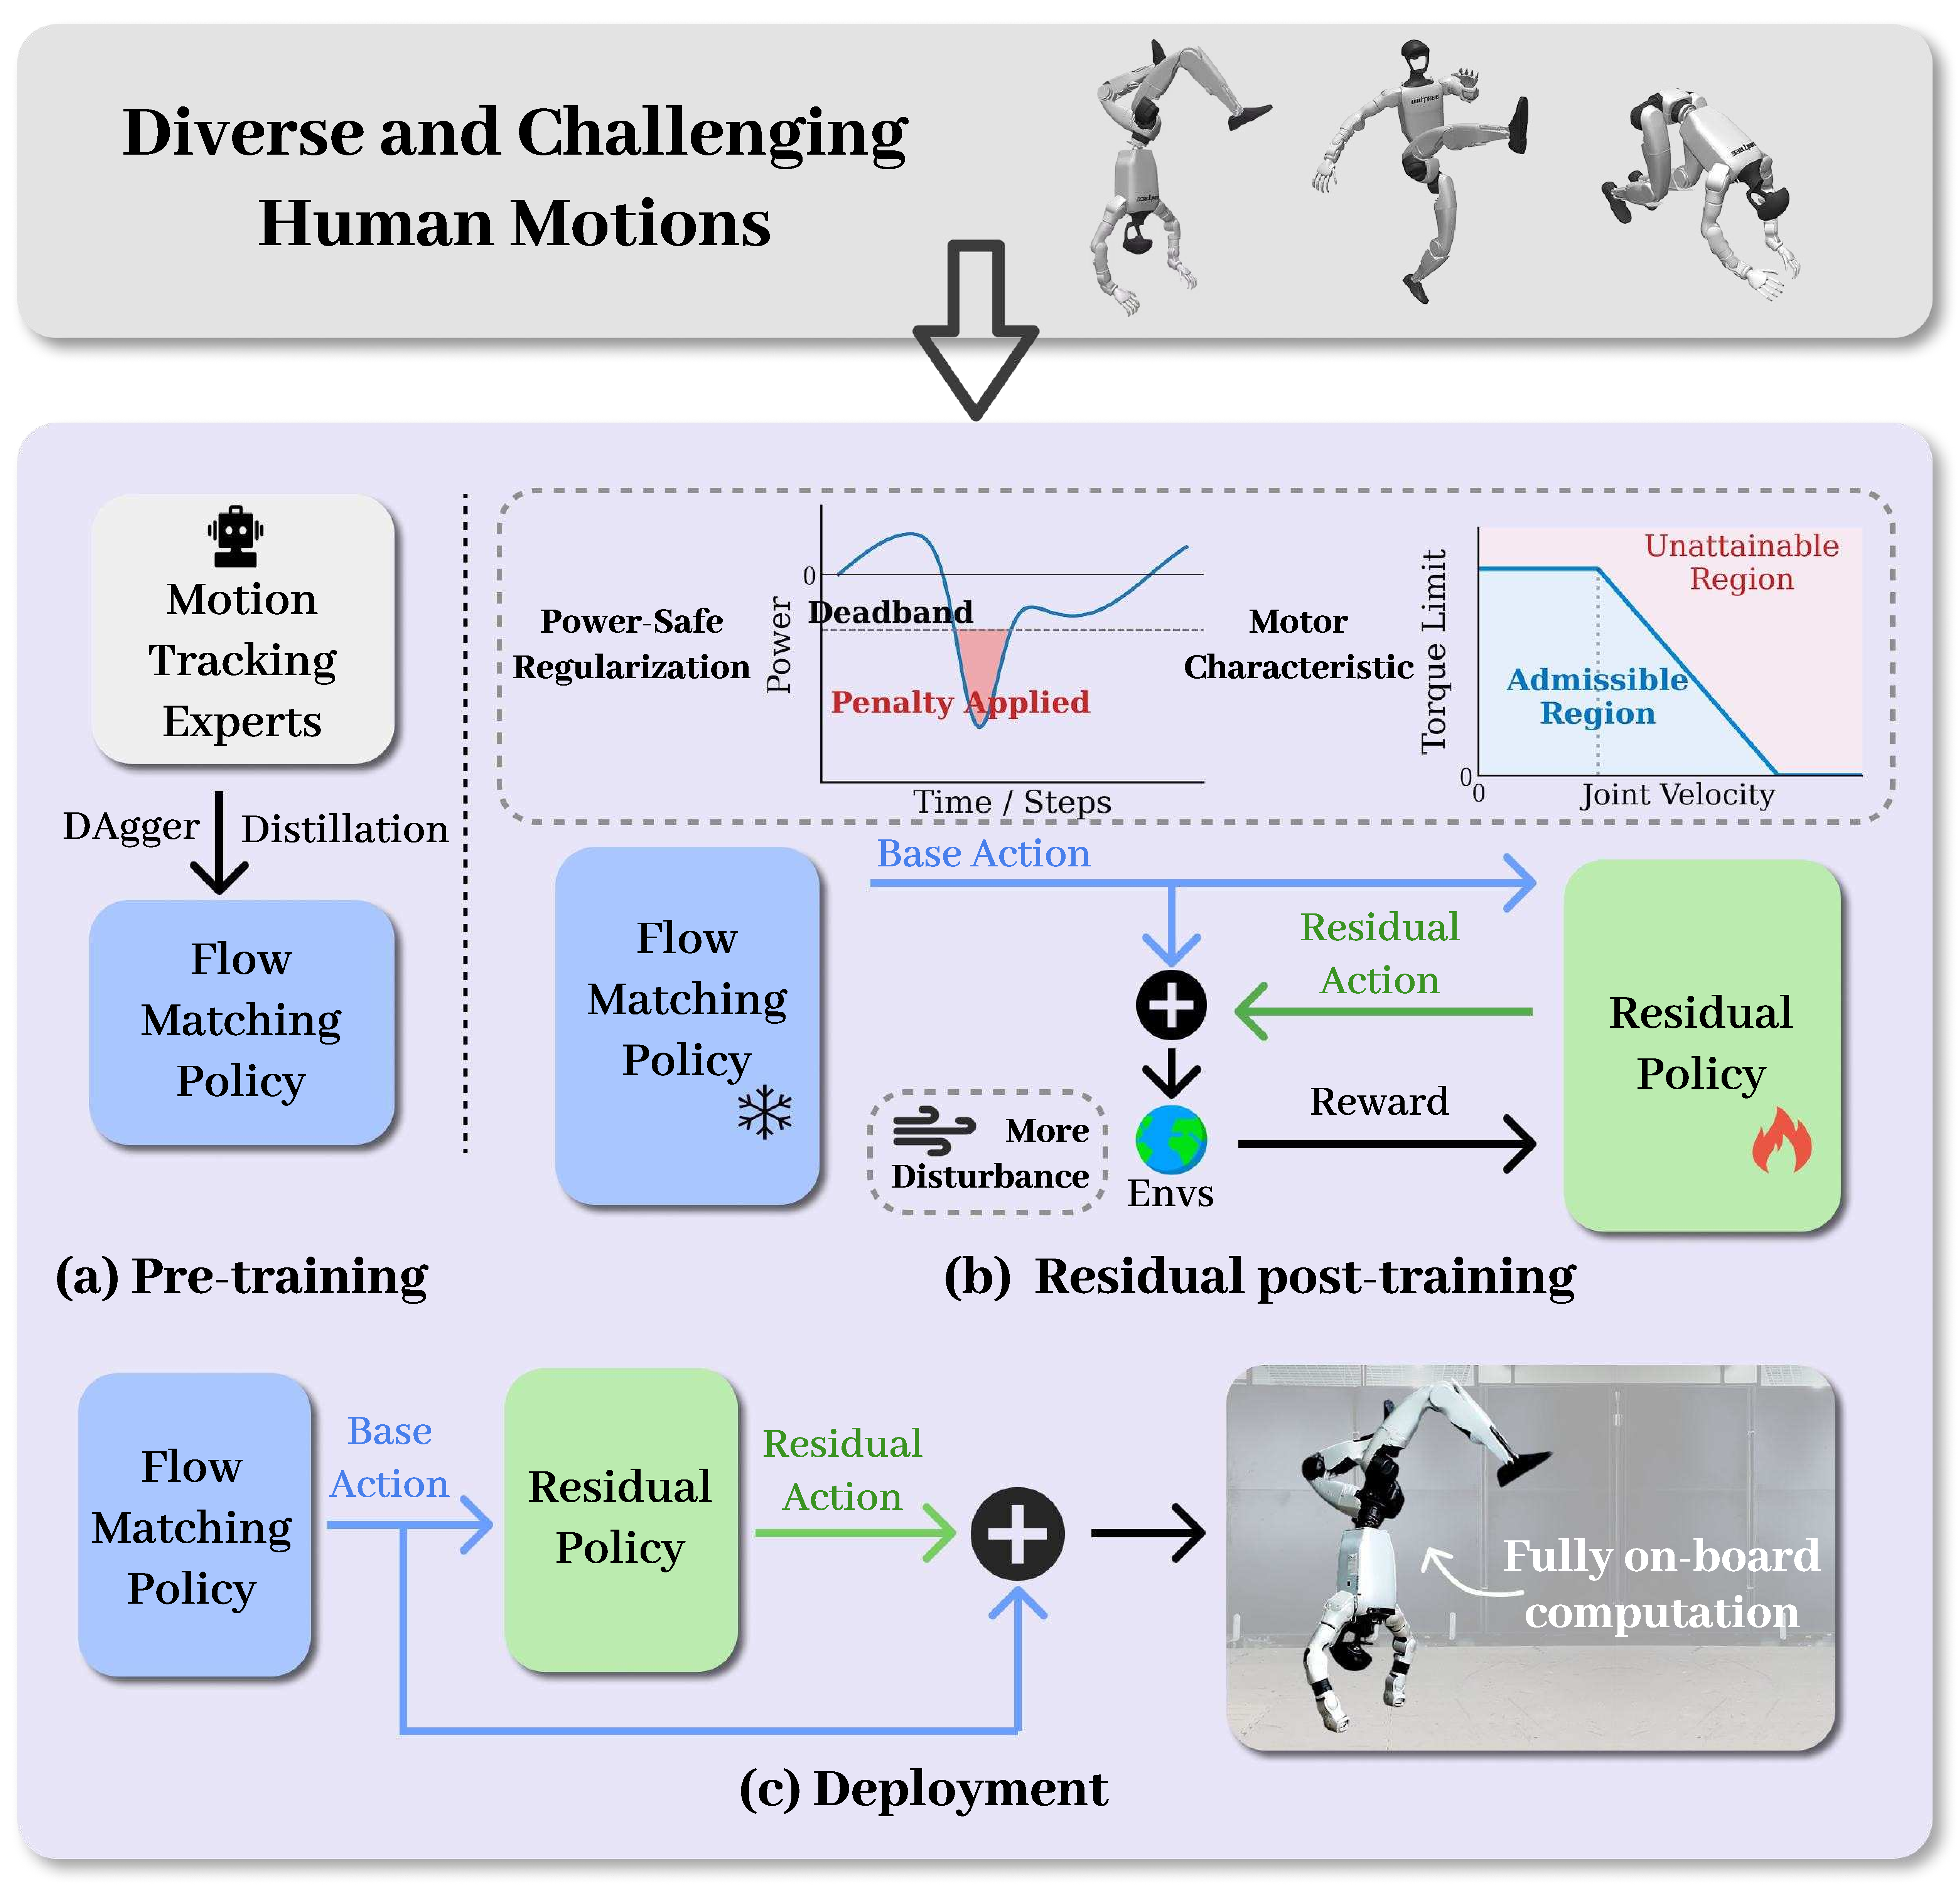
\includegraphics[width=.995\columnwidth]{figures/method_final.pdf}
\caption{\small \textbf{Overview of the \model.} (a) Pretraining phase: A unified base policy is trained via DAgger-based Flow Matching to aggregate diverse motion priors from different motion tracking experts. (b) Post-training phase: The base policy is frozen while a residual policy is optimized under stringent motor constraints, extensive domain randomization, and power-safety regularization to bridge the sim-to-real gap. (c) Onboard deployment: The whole inference pipeline is real-time and executed entirely onboard, facilitating robust and agile control in physical environments.}
\label{fig:method_overview}
\vspace{-17pt}
\end{figure}